\documentclass[a4paper, twocolumn]{ltjsarticle}
%preamble.tex

%LaTeXエンジン
\usepackage{luatexja}

%フォント
%\usepackage[ipaex]{luatexja-preset}

%図表
\usepackage{graphicx}
\usepackage{tikz}
\usepackage{multirow}
\usepackage{float}
\usepackage{wrapfig}

%数学
\usepackage{mathtools}
\usepackage{amsmath}

%科学
\usepackage{physics}
\usepackage{siunitx}
\usepackage[version=4]{mhchem}

%リンク
\usepackage{url}

%ハイパーリンク
\usepackage[unicode,hidelinks,pdfusetitle]{hyperref}

%余白
\usepackage[margin=12truemm]{geometry}

%枠付き
\usepackage{ascmac}
\usepackage{fancybox}

%%%%%%%%%%%%%%%%%%%%%%%%%%%%%%%%%%%%%%%%%%%%%%%%%
\begin{document}
\title{北海道大学理学部地球惑星科学科 オープンキャンパス\\クレーター形成実験 解説問題}
\date{\today}
\maketitle
\thispagestyle{empty}
%%%%%%%%%%%%%%%%%%%%%%%%%%%%%%%%%%%%%%%%%%%%%%%%%
今回のクレーターが半球であると近似してクレーター直径$D$と衝突エネルギー$E$の関係を求めてみよう。

砂の密度を$\rho$、重力加速度を$g$とする。クレーターをつくるためのエネルギーを、砂地の中の直径$D$の半球をその半径の分だけそのまま持ち上げるエネルギーで近似する。なぜならば、クレーターができるためには、半球を埋めていた物質がその半球の外に出ていかなければならないからである。そのエネルギーは、半球の質量と$g$と半球の半径の積で表される。おもりの衝突エネルギーがすべてこのエネルギーに変換されたと仮定すると次の等式が成り立つ。
\begin{equation}
    クレーターをつくるためのエネルギー = E
\end{equation}

以上のことからクレーターの直径$D$と衝突エネルギー$E$の関係式を求めよ。

※不明な点があれば遠慮なく担当者に質問してください。
\begin{figure}[H]
    \centering
    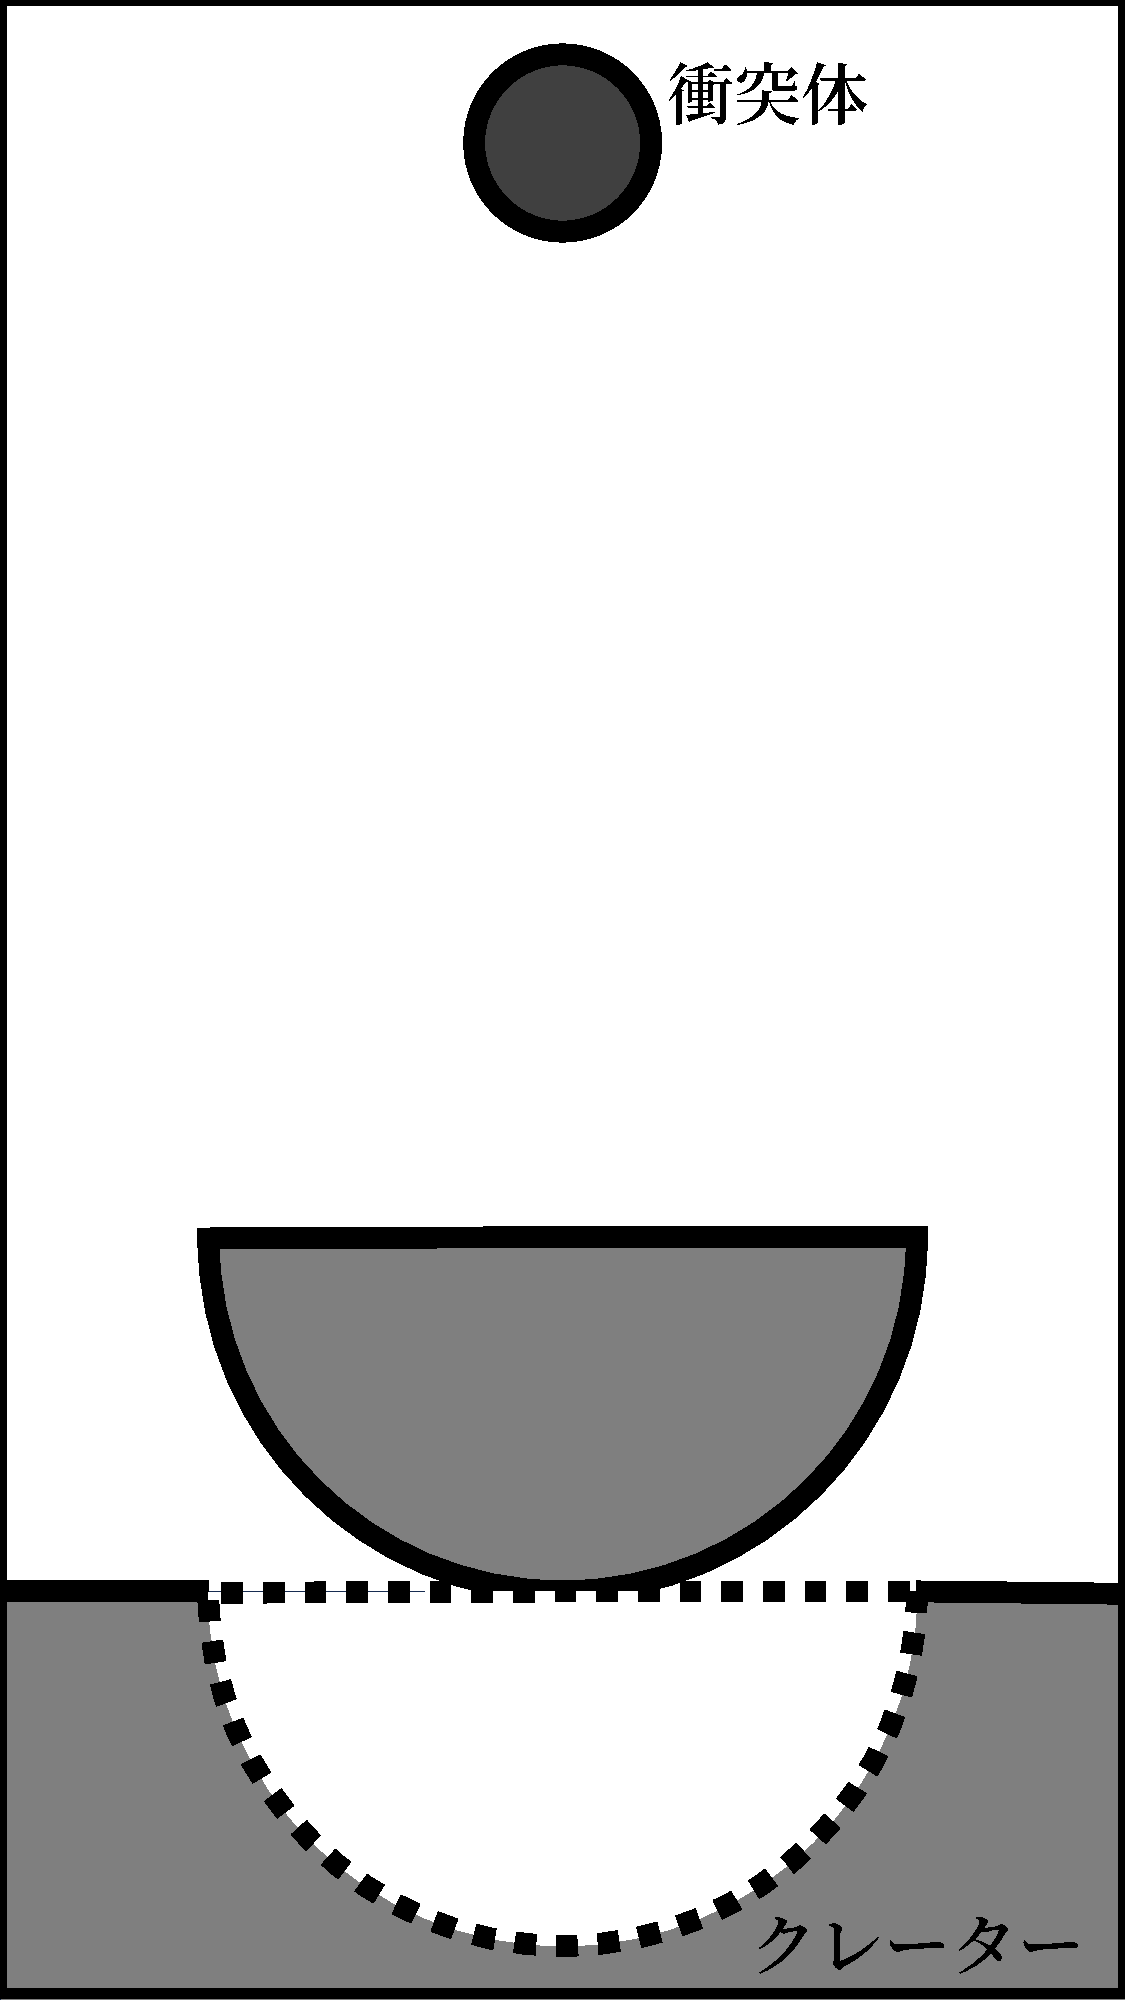
\includegraphics[height=13cm]{./figure/explanation_figure.pdf}
    \caption{参考図}
\end{figure}

(解答欄)
\end{document}
